\documentclass[12pt,letterpaper]{article}

%Packages
% \usepackage{textcomp}
% \usepackage{latexsym}
% \usepackage{url}
% \usepackage{epsfig}
% \usepackage{graphicx}
% \usepackage{amssymb}
% \usepackage{amsmath}
% \usepackage{mathtools}
% \usepackage{bm}
% \usepackage{array}
% \usepackage[version=3]{mhchem}
% \usepackage{ifthen}
% \usepackage{caption}
% \usepackage{amsthm}
% \usepackage{amstext}
% \usepackage{enumerate}
% \usepackage[osf]{mathpazo}
% \usepackage{dcolumn}

\usepackage{hyperref}
\usepackage{lineno}
\usepackage{pdflscape}
\usepackage{mathtools}
\usepackage[osf]{mathpazo}
\usepackage{fullpage}
\usepackage{float}

\pagenumbering{arabic}


%---------------------------------------------
%
%       START
%
%---------------------------------------------

\begin{document}
%Running head
\begin{flushright}
Version dated: \today
\end{flushright}

\bigskip
\medskip
\begin{center}

\noindent{\Large \bf Innovation and elaboration on the avian tree of life}
\bigskip

\noindent {\normalsize \sc Thomas Guillerme$^{1,*}$, Natalie Cooper$^{2}$, Andrew P. Beckerman$^{1}$, and Gavin H. Thomas$^{1}$}\\
\noindent {\small \it 
$^1$chool of Biosciences, University of Sheffield, heffield, S10 2TN, United Kingdom.\\
$^2$Natural History Museum, Cromwell Road, London, SW75BD, United Kingdom.\\}

\end{center}
\medskip
\noindent{*\bf Corresponding author.} \textit{guillert@tcd.ie}\\ 
\vspace{1in}

%Line numbering
\modulolinenumbers[1]
\linenumbers

%---------------------------------------------
%
%       ABSTRACT
%
%---------------------------------------------

\noindent (Keywords: )\\

\vspace{1.5in}

\newpage 

%---------------------------------------------
%
%       INTRODUCTION
%
%---------------------------------------------
 blabalbal \cite{dispRity}


\begin{figure}
\centering
   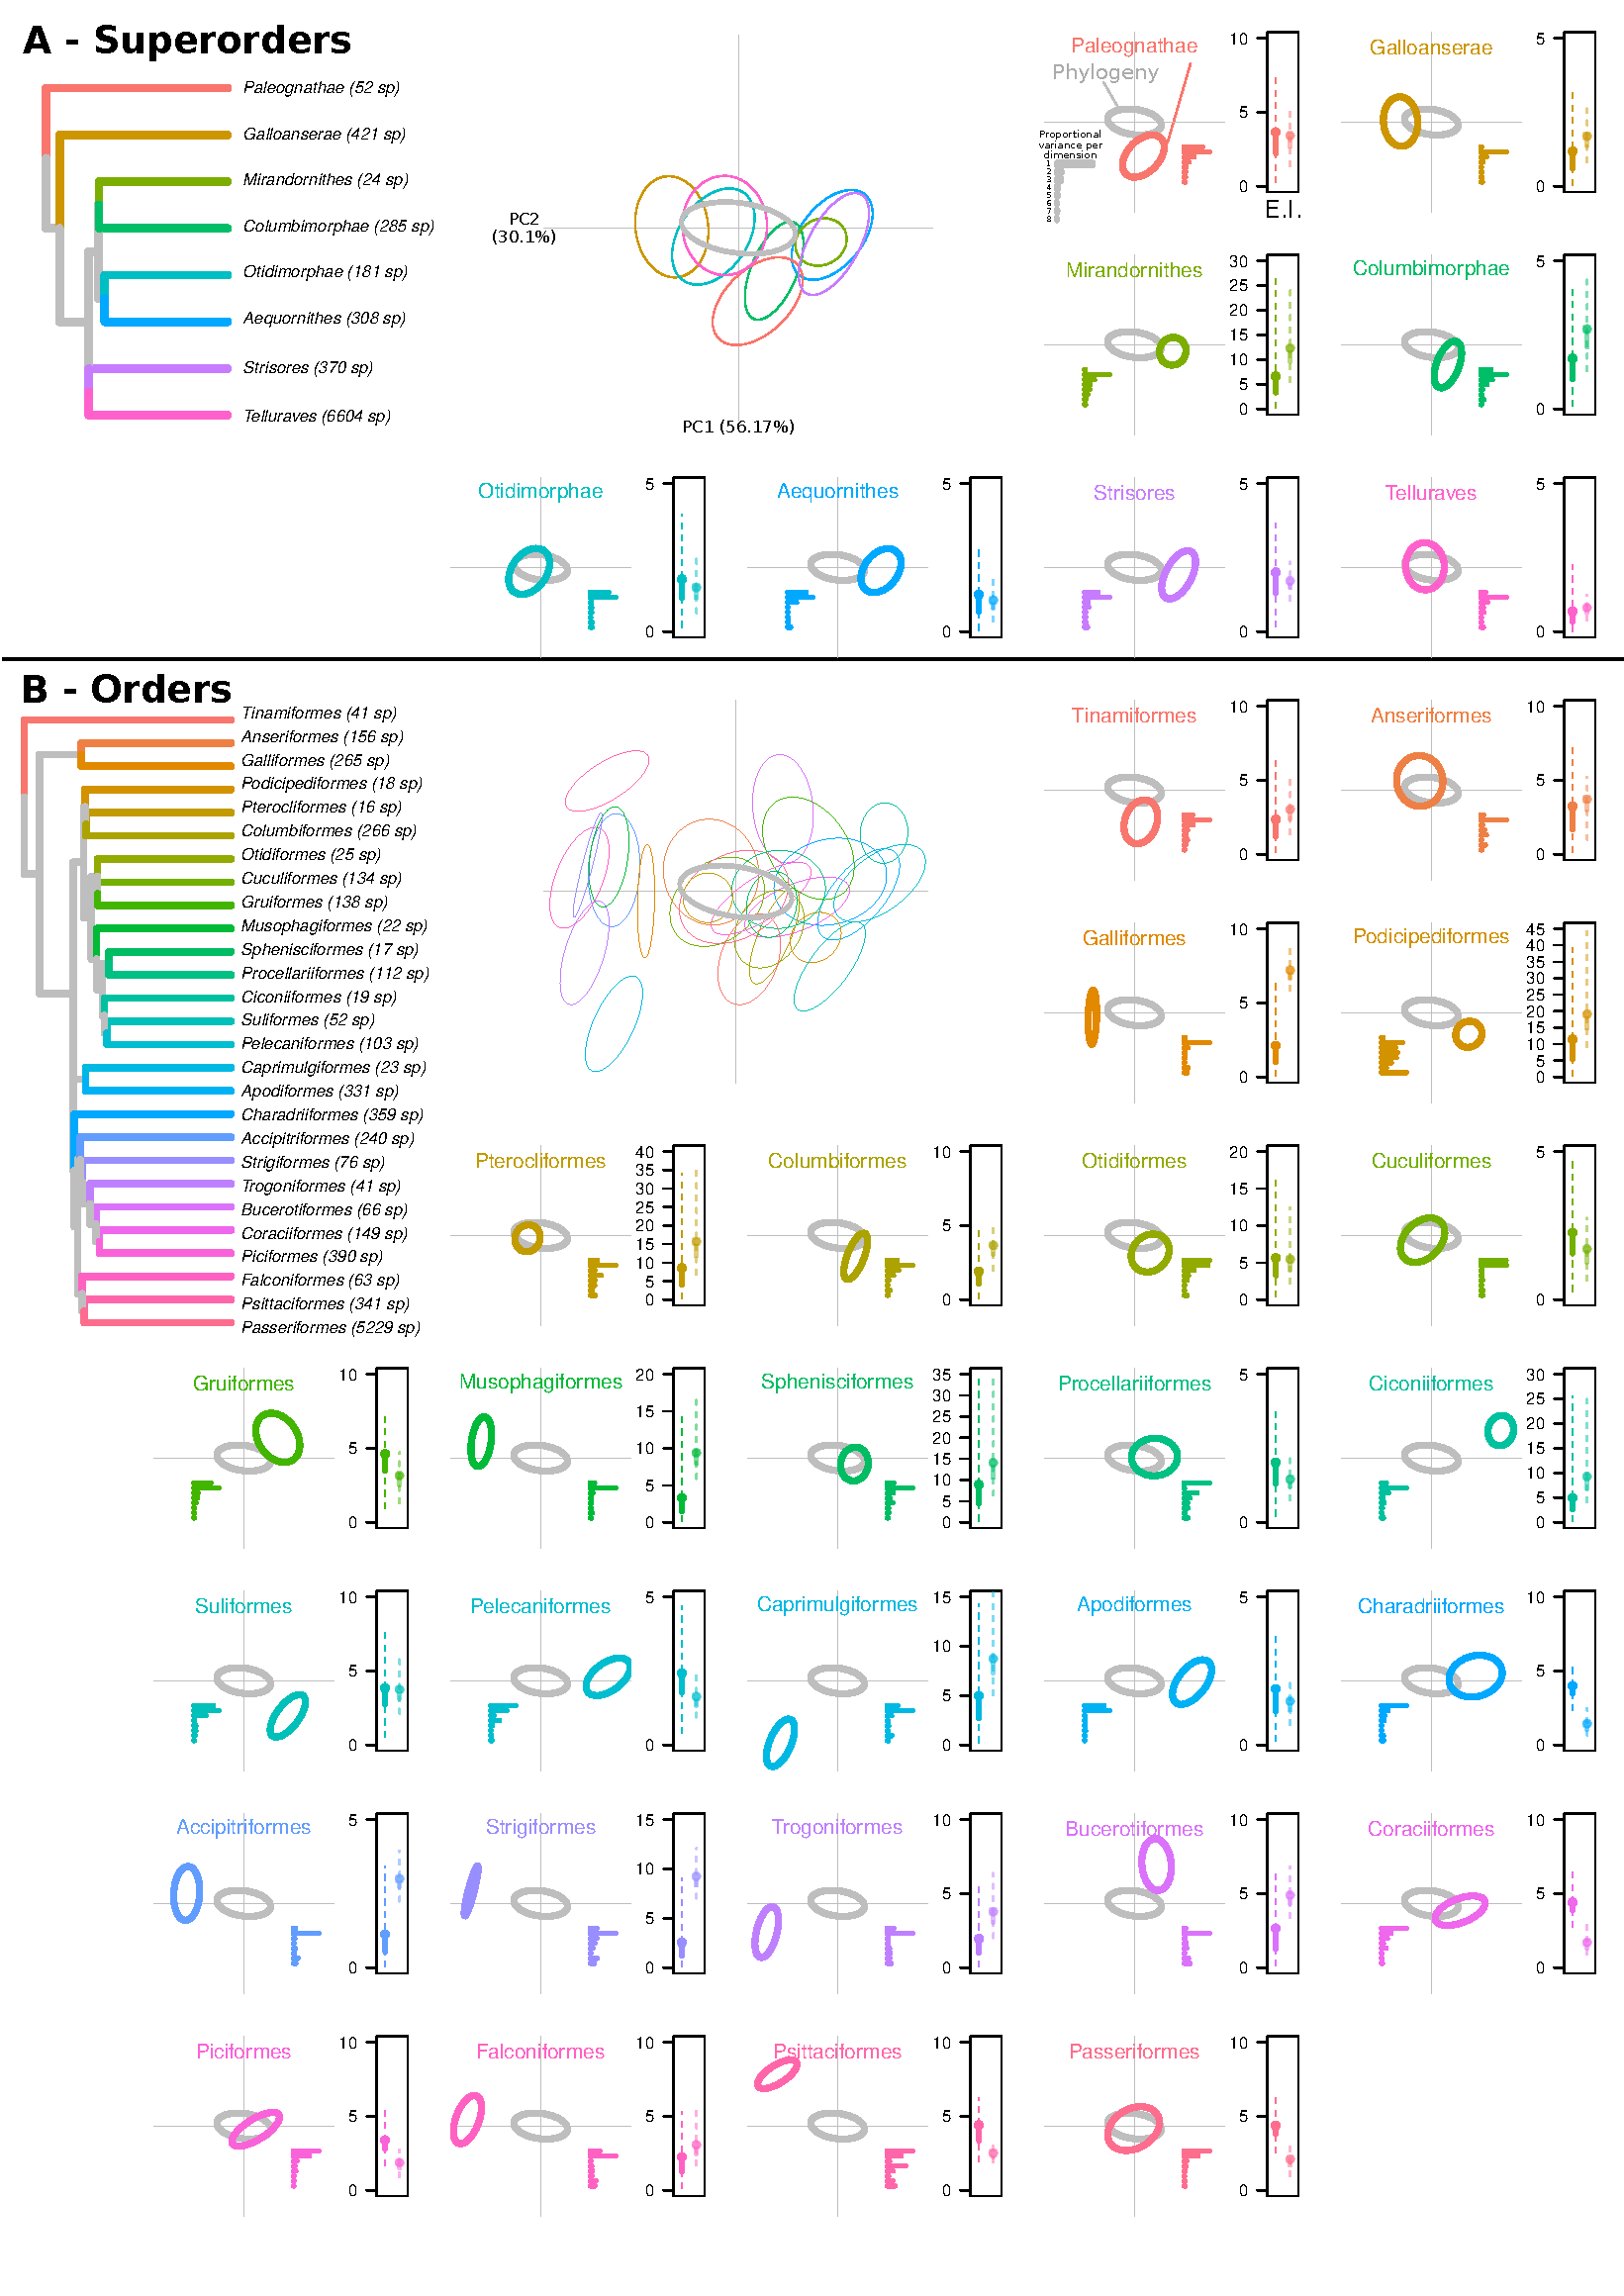
\includegraphics[width=1\textwidth]{Figures/ellipses.pdf}
\caption{.}
\label{Fig:ellipses}
\end{figure}


\begin{figure}[!htbp]
\centering
   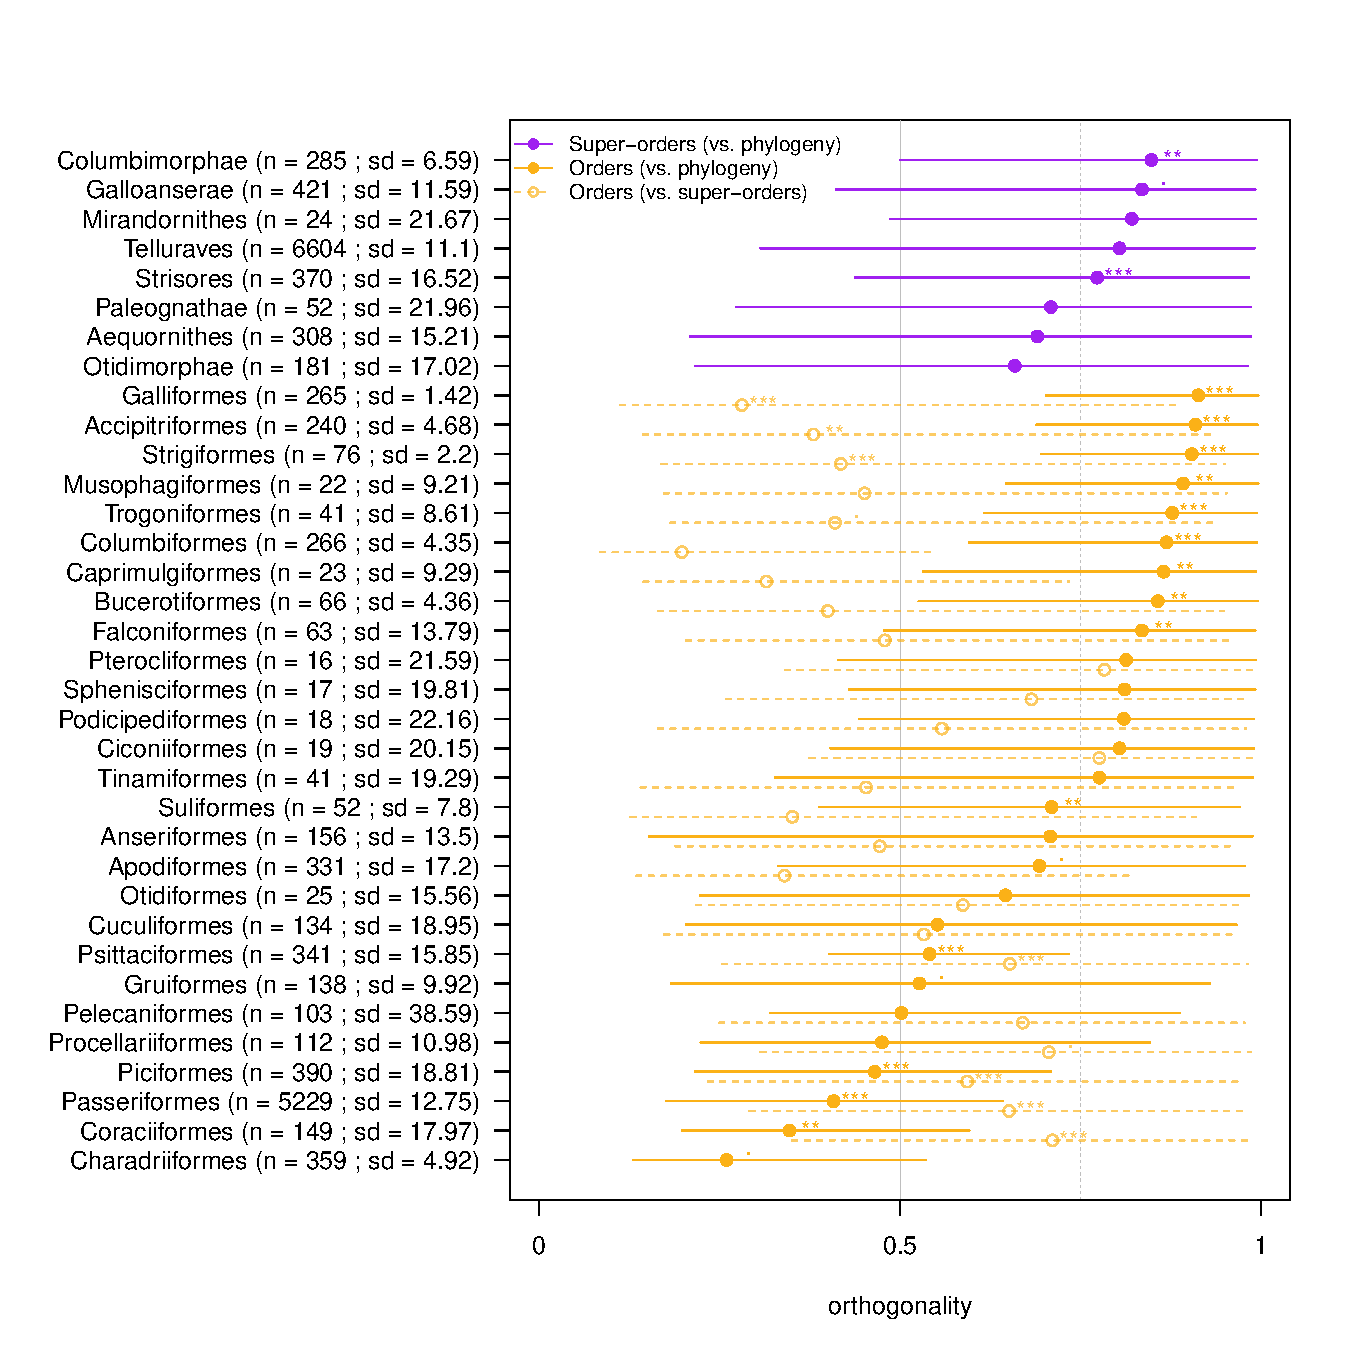
\includegraphics[width=0.9\textwidth]{Figures/orthogonality_results.pdf}
\caption{.}
\label{Fig:orthogonality}
\end{figure}


\begin{figure}[!htbp]
\centering
   % \includegraphics[width=0.9\textwidth]{Figures/phylogenys.pdf}
\caption{.}
\label{Fig:phylogeny}
\end{figure}


\begin{figure}[!htbp]
\centering
   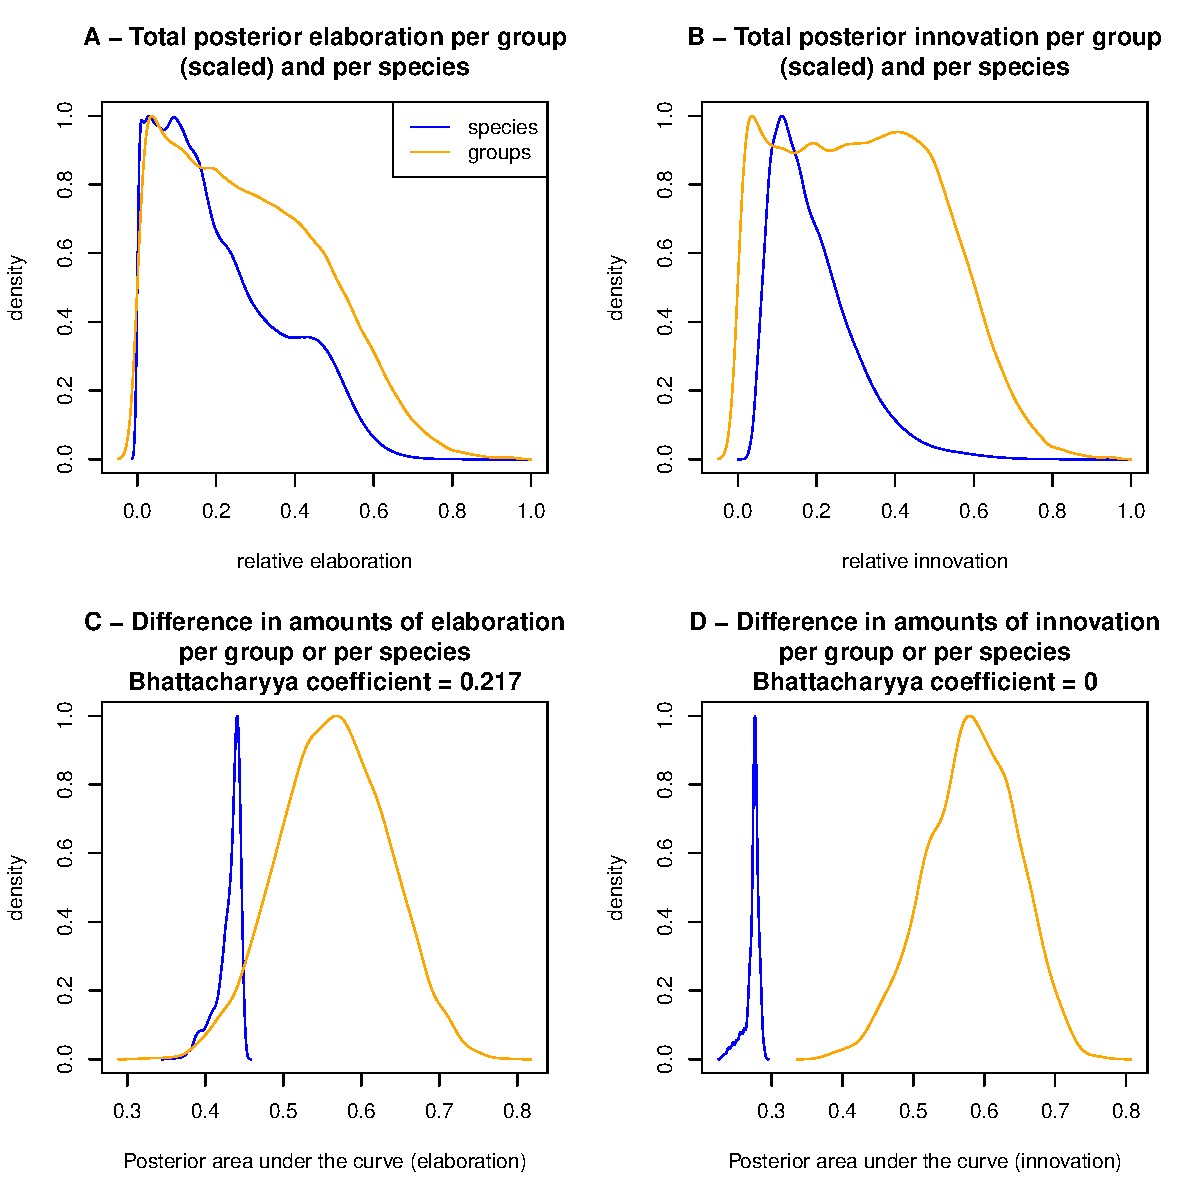
\includegraphics[width=0.9\textwidth]{Figures/relative_EI.pdf}
\caption{.}
\label{Fig:relative_EI}
\end{figure}




\bibliographystyle{naturemag}
\bibliography{References}


\end{document}